% Options for packages loaded elsewhere
\PassOptionsToPackage{unicode}{hyperref}
\PassOptionsToPackage{hyphens}{url}
%
\documentclass[
]{book}
\usepackage{lmodern}
\usepackage{amssymb,amsmath}
\usepackage{ifxetex,ifluatex}
\ifnum 0\ifxetex 1\fi\ifluatex 1\fi=0 % if pdftex
  \usepackage[T1]{fontenc}
  \usepackage[utf8]{inputenc}
  \usepackage{textcomp} % provide euro and other symbols
\else % if luatex or xetex
  \usepackage{unicode-math}
  \defaultfontfeatures{Scale=MatchLowercase}
  \defaultfontfeatures[\rmfamily]{Ligatures=TeX,Scale=1}
\fi
% Use upquote if available, for straight quotes in verbatim environments
\IfFileExists{upquote.sty}{\usepackage{upquote}}{}
\IfFileExists{microtype.sty}{% use microtype if available
  \usepackage[]{microtype}
  \UseMicrotypeSet[protrusion]{basicmath} % disable protrusion for tt fonts
}{}
\makeatletter
\@ifundefined{KOMAClassName}{% if non-KOMA class
  \IfFileExists{parskip.sty}{%
    \usepackage{parskip}
  }{% else
    \setlength{\parindent}{0pt}
    \setlength{\parskip}{6pt plus 2pt minus 1pt}}
}{% if KOMA class
  \KOMAoptions{parskip=half}}
\makeatother
\usepackage{xcolor}
\IfFileExists{xurl.sty}{\usepackage{xurl}}{} % add URL line breaks if available
\IfFileExists{bookmark.sty}{\usepackage{bookmark}}{\usepackage{hyperref}}
\hypersetup{
  pdftitle={Tools for Working with Data - 327},
  pdfauthor={Nicole Sorhagen, Ph.D.},
  hidelinks,
  pdfcreator={LaTeX via pandoc}}
\urlstyle{same} % disable monospaced font for URLs
\usepackage{longtable,booktabs}
% Correct order of tables after \paragraph or \subparagraph
\usepackage{etoolbox}
\makeatletter
\patchcmd\longtable{\par}{\if@noskipsec\mbox{}\fi\par}{}{}
\makeatother
% Allow footnotes in longtable head/foot
\IfFileExists{footnotehyper.sty}{\usepackage{footnotehyper}}{\usepackage{footnote}}
\makesavenoteenv{longtable}
\usepackage{graphicx,grffile}
\makeatletter
\def\maxwidth{\ifdim\Gin@nat@width>\linewidth\linewidth\else\Gin@nat@width\fi}
\def\maxheight{\ifdim\Gin@nat@height>\textheight\textheight\else\Gin@nat@height\fi}
\makeatother
% Scale images if necessary, so that they will not overflow the page
% margins by default, and it is still possible to overwrite the defaults
% using explicit options in \includegraphics[width, height, ...]{}
\setkeys{Gin}{width=\maxwidth,height=\maxheight,keepaspectratio}
% Set default figure placement to htbp
\makeatletter
\def\fps@figure{htbp}
\makeatother
\setlength{\emergencystretch}{3em} % prevent overfull lines
\providecommand{\tightlist}{%
  \setlength{\itemsep}{0pt}\setlength{\parskip}{0pt}}
\setcounter{secnumdepth}{5}
\usepackage{booktabs}
\usepackage{amsthm}
\makeatletter
\def\thm@space@setup{%
  \thm@preskip=8pt plus 2pt minus 4pt
  \thm@postskip=\thm@preskip
}
\makeatother
\usepackage[]{natbib}
\bibliographystyle{apalike}

\title{Tools for Working with Data - 327}
\author{Nicole Sorhagen, Ph.D.}
\date{2020-08-11}

\begin{document}
\maketitle

{
\setcounter{tocdepth}{1}
\tableofcontents
}
\hypertarget{about-this-book}{%
\chapter{About this book}\label{about-this-book}}

This book describes how to use R as a tool to work with data.

R statistics is becoming increasingly popular for data management and analysis due to its accessibility and versatility. For example, R can produce records of data analyses, which is consistent with the growing move towards reproducible and open science within the field of psychology. R statistics is also known for making elegant graphs, which can help develop data visualization skills. Because it is open-sourced it is extremely flexible - people create and share packages that make certain aspects of data analysis easy.

R is a programming language. Although learning a programming language can seem a bit intimidating, there are many benefits to trying to figure it out. Mastering the basics of R could be useful for your future coursework, as well as for data management and analysis needs outside the classroom (independent research, future employment, etc.). That is to say, learning the basics of a programming language is a highly transferable skill.

The R programming language can be used within the R software as well as other programs. RStudio is a IDE (integrated development environment) and was designed to make the use of the R programming language more user friendly.

R, and its companion program RStudio, are free and available in PC, Mac, and Linux versions, so students can have it on their own computer - eliminating the need to visit computer labs or to buy student versions of expensive software. R can be downloaded from the CRAN (Comprehensive R Archive Network) (\url{https://www.r-project.org/}). Rstudio can be found here: \url{https://rstudio.com/}.

While you are welcome to download R and Rstudio on your personal computer, you do not have to for this course. We will be using Rstudio on a website called Rstudio cloud for class work (this is discussed in more detail in the next chapter). So I am not going to go into detail on downloading the programs on to your computer here. Please email me if you are interested in this and are having a hard time figuring it out.

Finally, please note that I will be updating this book over the course of the semester.

This work is licensed under a Creative Commons Attribution-NoDerivatives 4.0 International License.

\hypertarget{set-up-project-on-rstudio-cloud}{%
\chapter{Set up project on Rstudio Cloud}\label{set-up-project-on-rstudio-cloud}}

We will use Rstudio cloud on this website: \url{https://rstudio.cloud}.

You must first make an Rstudio account by clicking the sign up button in the top right corner. (this is free)


\includegraphics{img/signup.png}

Then join our shared RStudio cloud workspace with the link that I sent you in the email titled `Rstudio cloud shared workspace'.

\textbf{You MUST join our shared workspace.} I will be checking your work through this shared RStudio cloud workspace. Within this shared workspace, I will be able to see everyone's project, but you will only be able to see your project and my project.

Once you are in your Rstudio Cloud account\ldots{}

Expand the R studio cloud options by clicking on the 3 lines in the top left corner.

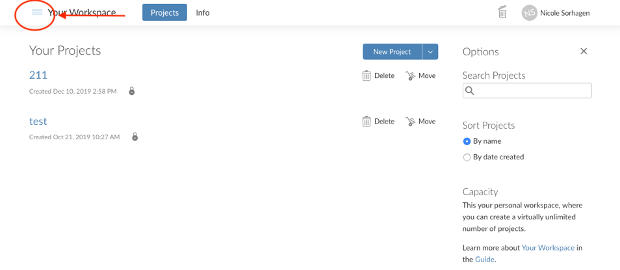
\includegraphics{img/Picture1.png}

Then select our course (which will be titled the name of course and the semester). If you cannot see this option -- then you have not been added to our shared workspace.

Once you are in the shared the classes workspace, open a new project.

Call this project your last name by clicking on the box that says `Untitled Project' and typing your last name.

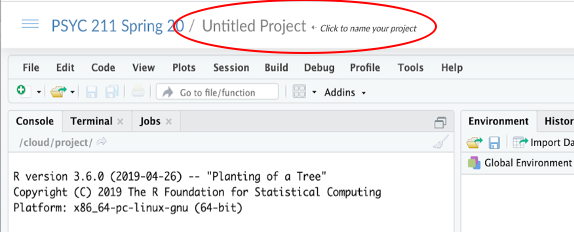
\includegraphics{img/Projname.png}

\hypertarget{introduction}{%
\chapter{Introduction}\label{introduction}}

This chapter introduces the Rstudio cloud environment and describes how to import data into the RStudio cloud.

R cannot handle typos and is case sensitive (`Gender' is not the same as `gender'). If your code will not run check for typos and caps. Related to this point, do not be afraid to copy and paste with using R. I often copy and paste code and replace variable or dataset names as needed. (This is one of the few times in education where copy and paste is OK!)

\hypertarget{layout-of-rstudio-cloud}{%
\section{Layout of Rstudio cloud}\label{layout-of-rstudio-cloud}}

Rstudio has four panes: the console panel, the script panel, the environment and history panel, and the files and plots panel. Each will be describe in turn next.

\hypertarget{console}{%
\subsection{Console}\label{console}}

The console panel of R studio is where you can type commands and where you will see the output of commands.

In its most basic form, you can think of R as a fancy calculator.

For example:

In the console type \texttt{2+2} and then press RETURN on your keyboard. The answer `4' will apear on the next line.

The \texttt{\textgreater{}} in the last line of the console means that the console is ready for a command (see red circle in the picture above).

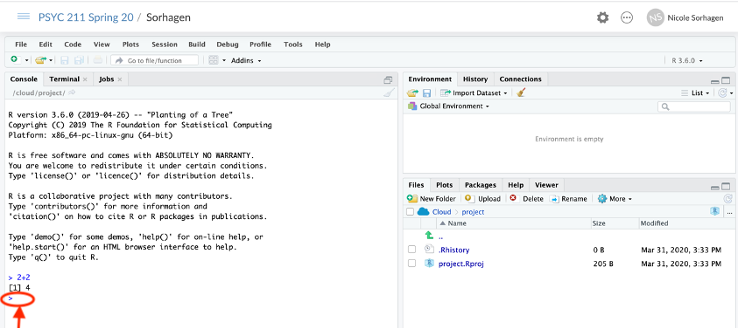
\includegraphics{img/twoplus.png}

If \texttt{\textgreater{}} is missing from the last line, it means that R is waiting for you to complete a command.

For example, type \texttt{1+} in the console and then hit enter.

The plus sign means the command is incomplete.

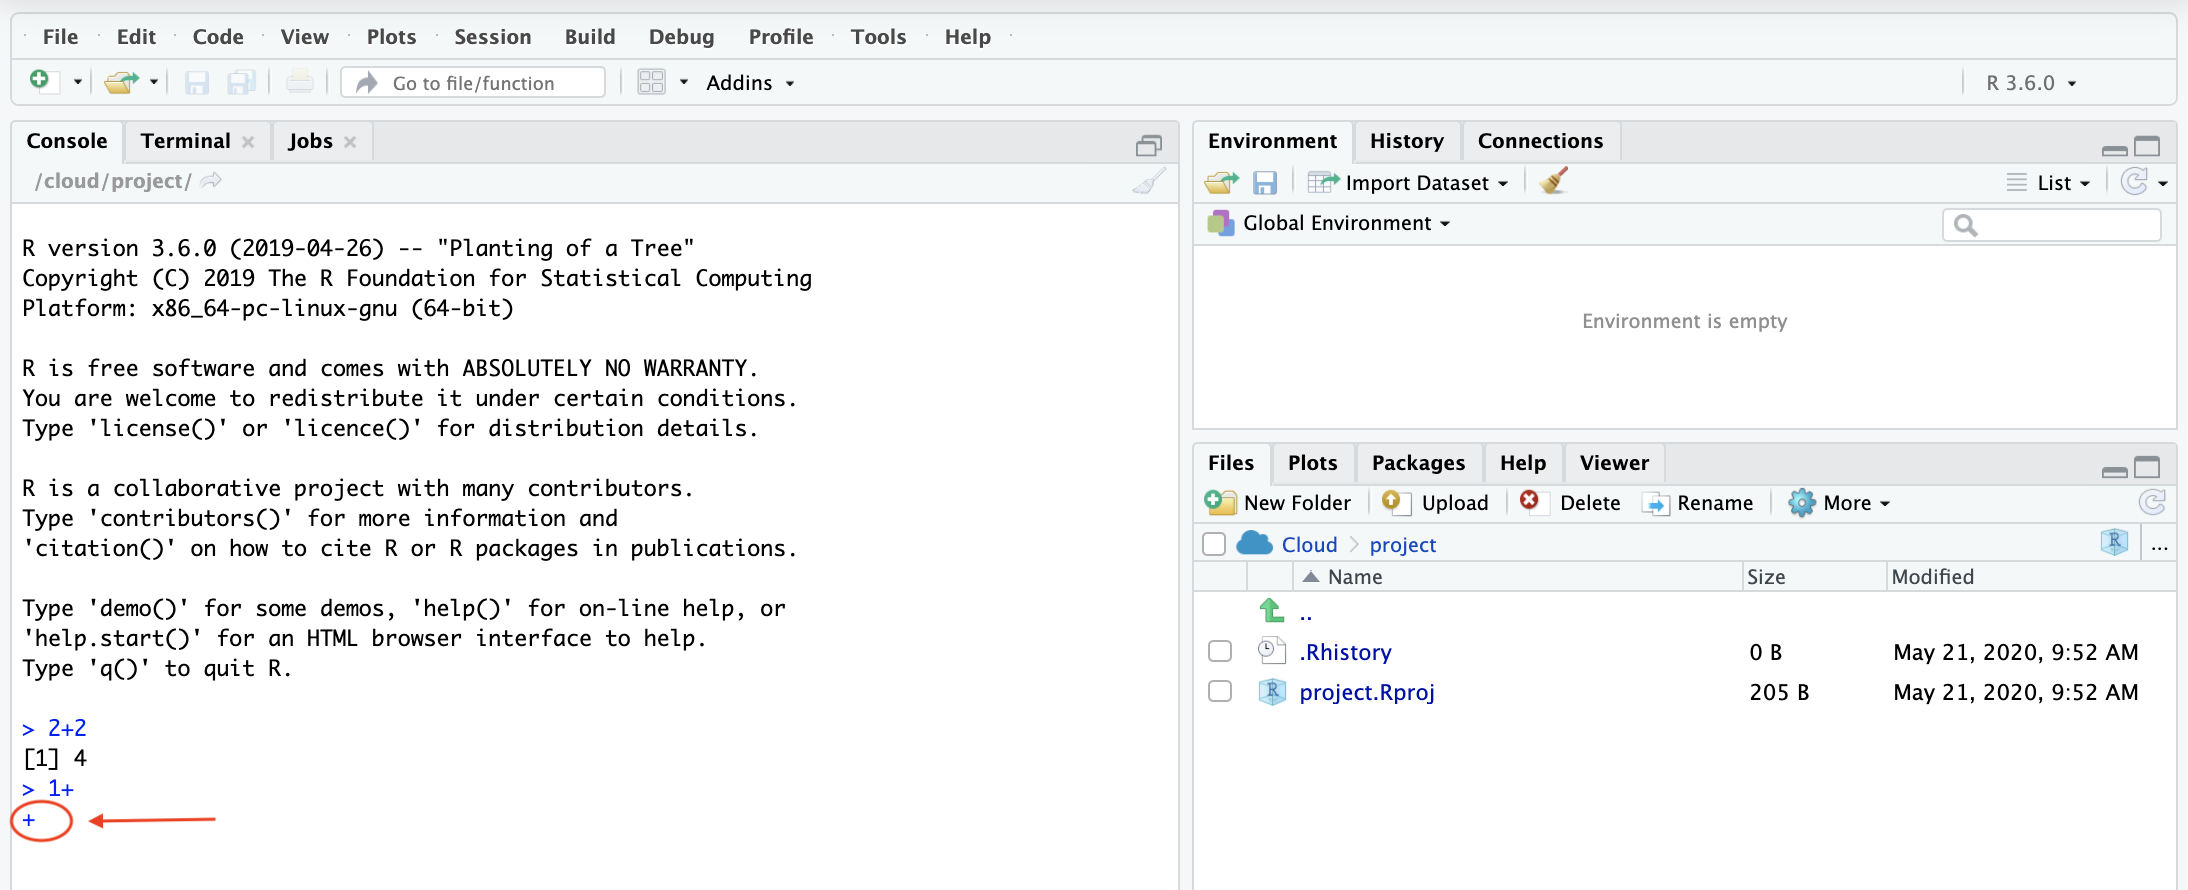
\includegraphics{img/waiting.png}

Push the \textbf{ESC} button on your keyboard to get back to the command prompt.

\hypertarget{script}{%
\subsection{Script}\label{script}}

One of the benefits of using R is that you can save a record of your work using scripts. Records of your work allow you to easily start and stop an assignment or research project. You can pick up where you left off whether it is 20 minutes later or 2 years later. It also lets you share with others -- from professors, to collaborators, to peer reviewers.

To create a new script, go to the top bar menu:

\textbf{FILE -\textgreater{} NEW FILE -\textgreater{} R SCRIPT}

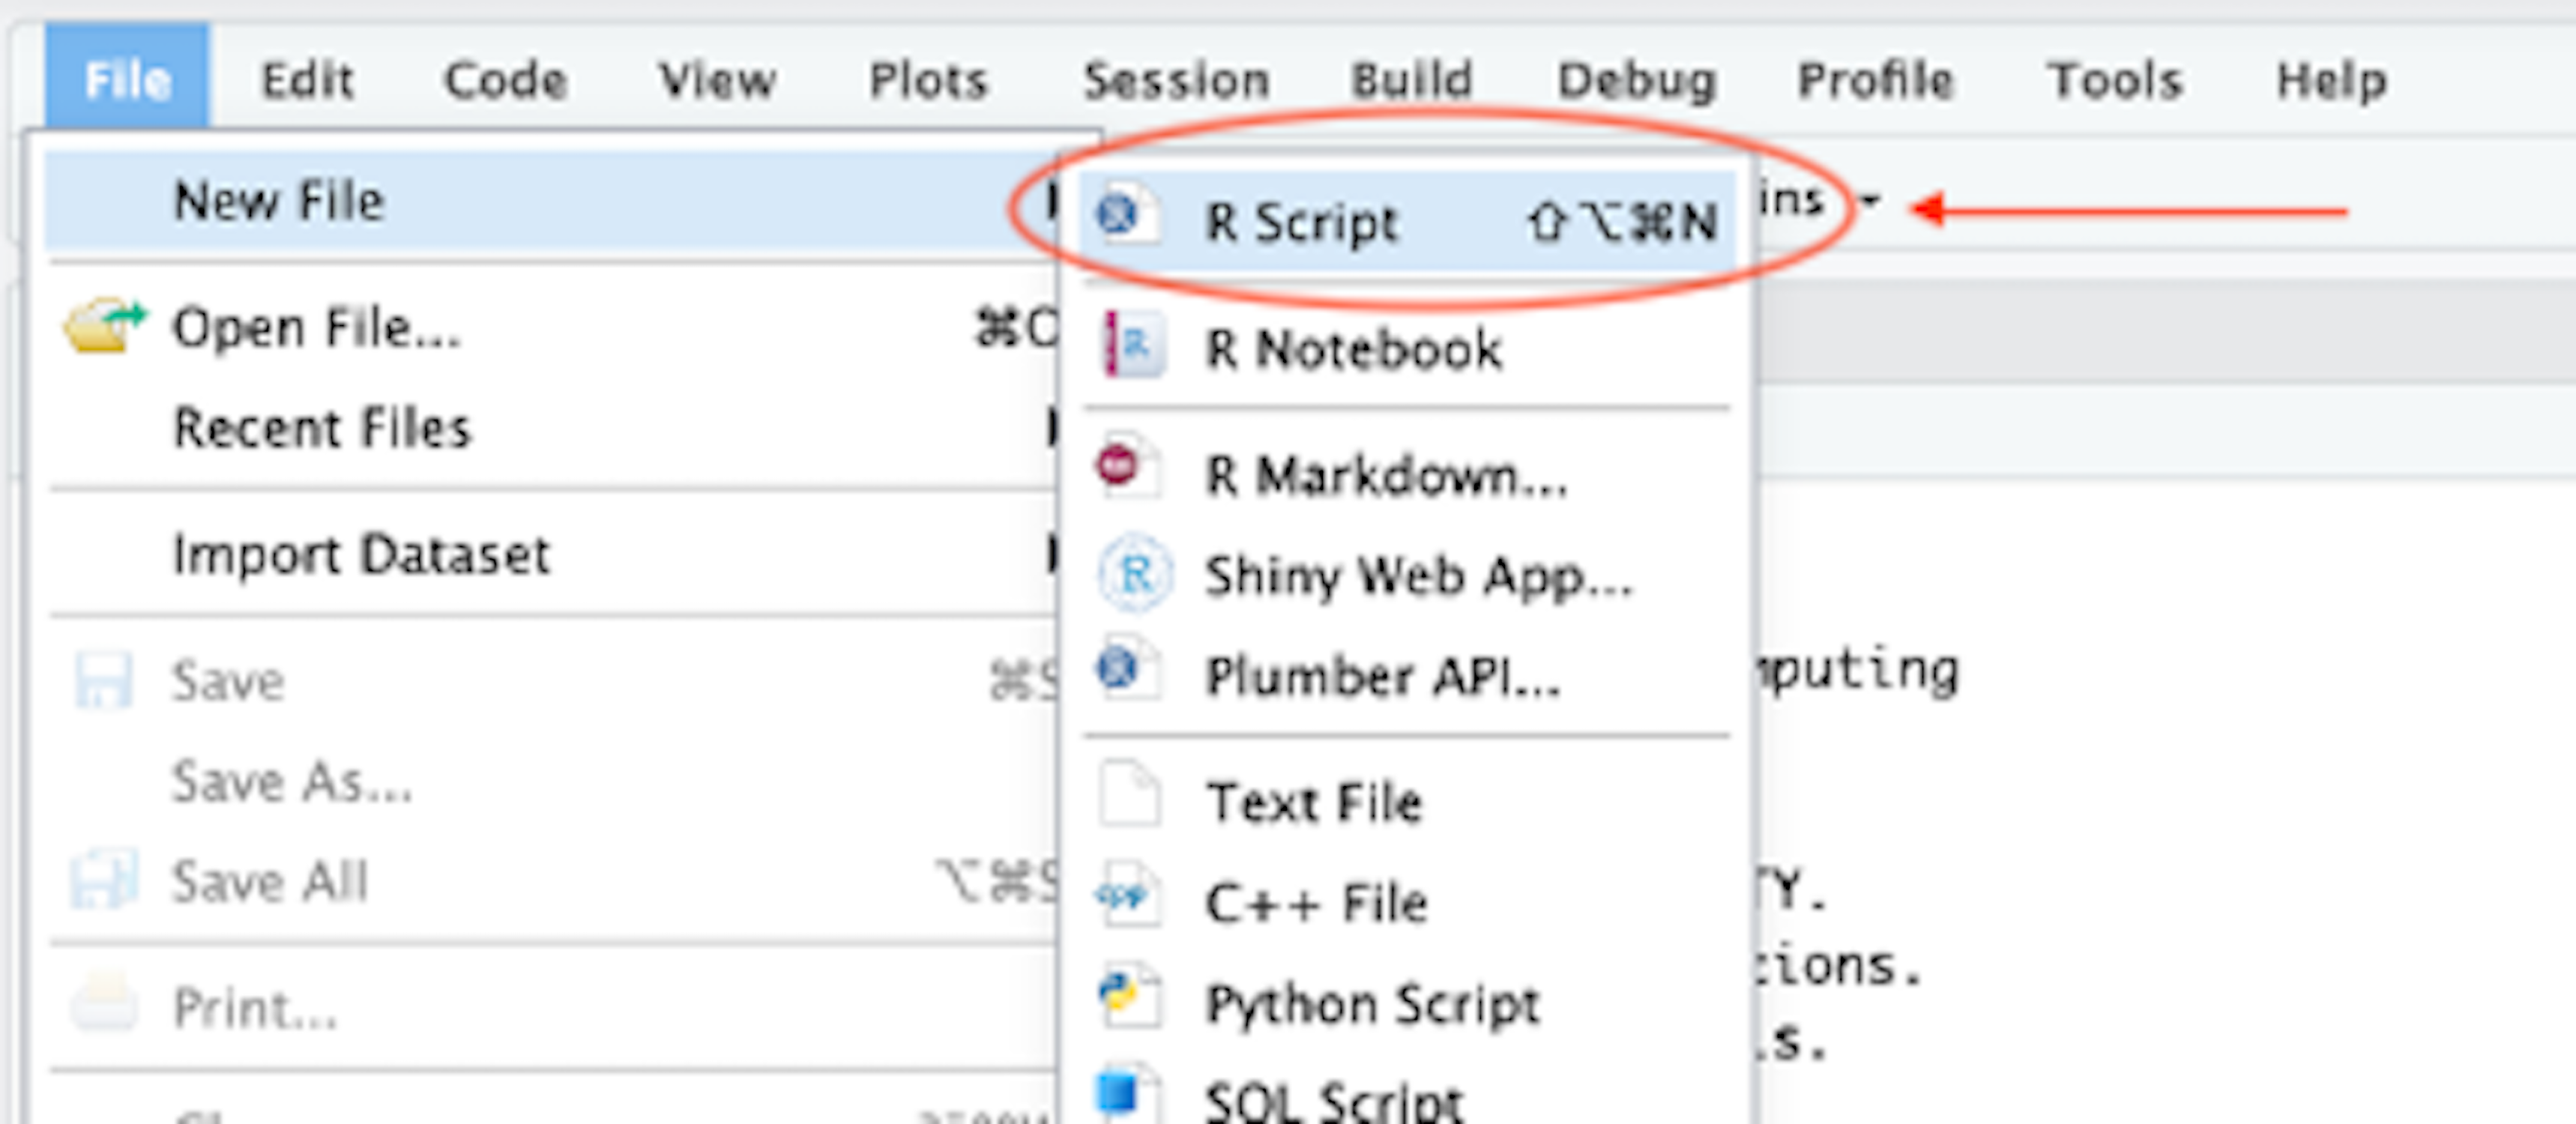
\includegraphics{img/newscript.png}

A new script will open in the top left of the RStudio platform.

\textbf{You should run code from scripts}

Scripts are similar to running command in the console (this is what you did in the last section).

For example, type \texttt{5+5} in the script panel.

In order to run command in a script you should click the run button while the cursor is in the code or the code is selected. You can also run the code by pressing the COMMAND and RETURN keys on your keyboard at the same time (the ALT and RETURN key on a pc).

After the code is run, the results will automatically appear the in console (see red arrow in the picture below).

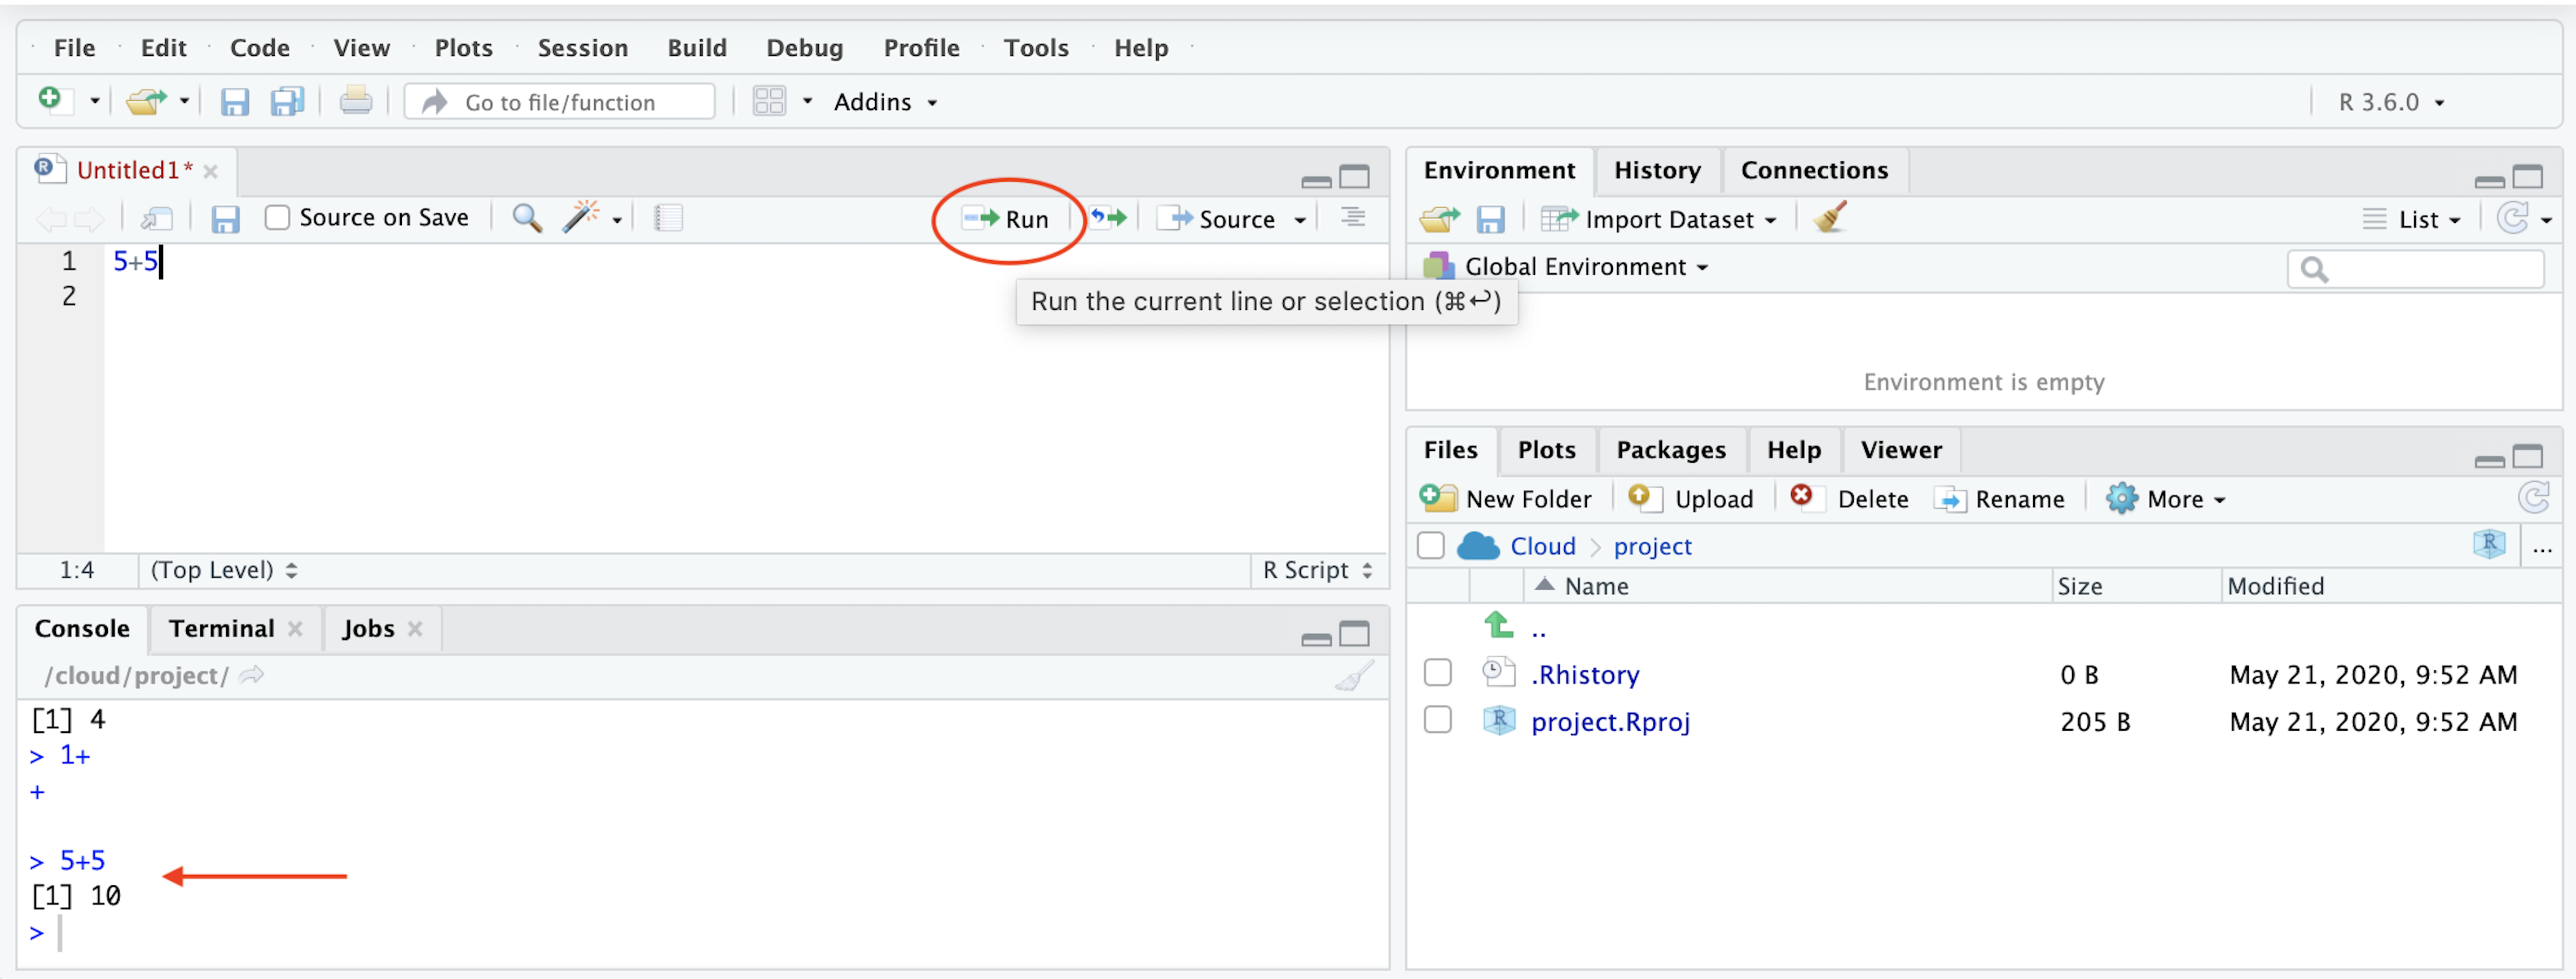
\includegraphics{img/script.png}

In order to use the script again you must \textbf{save} it.

From the drop-down menu select:

\textbf{FILE -\textgreater{} SAVE AS}

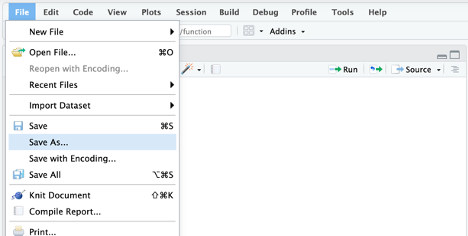
\includegraphics{img/savescript.png}

Type \textbf{lab 1} into the file name box. And then click the SAVE button.

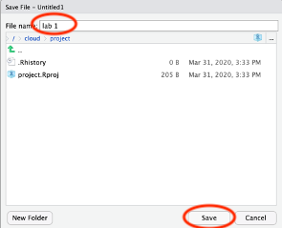
\includegraphics{img/savescript2.png}

Your file should now be listed in the files window in the bottom right.

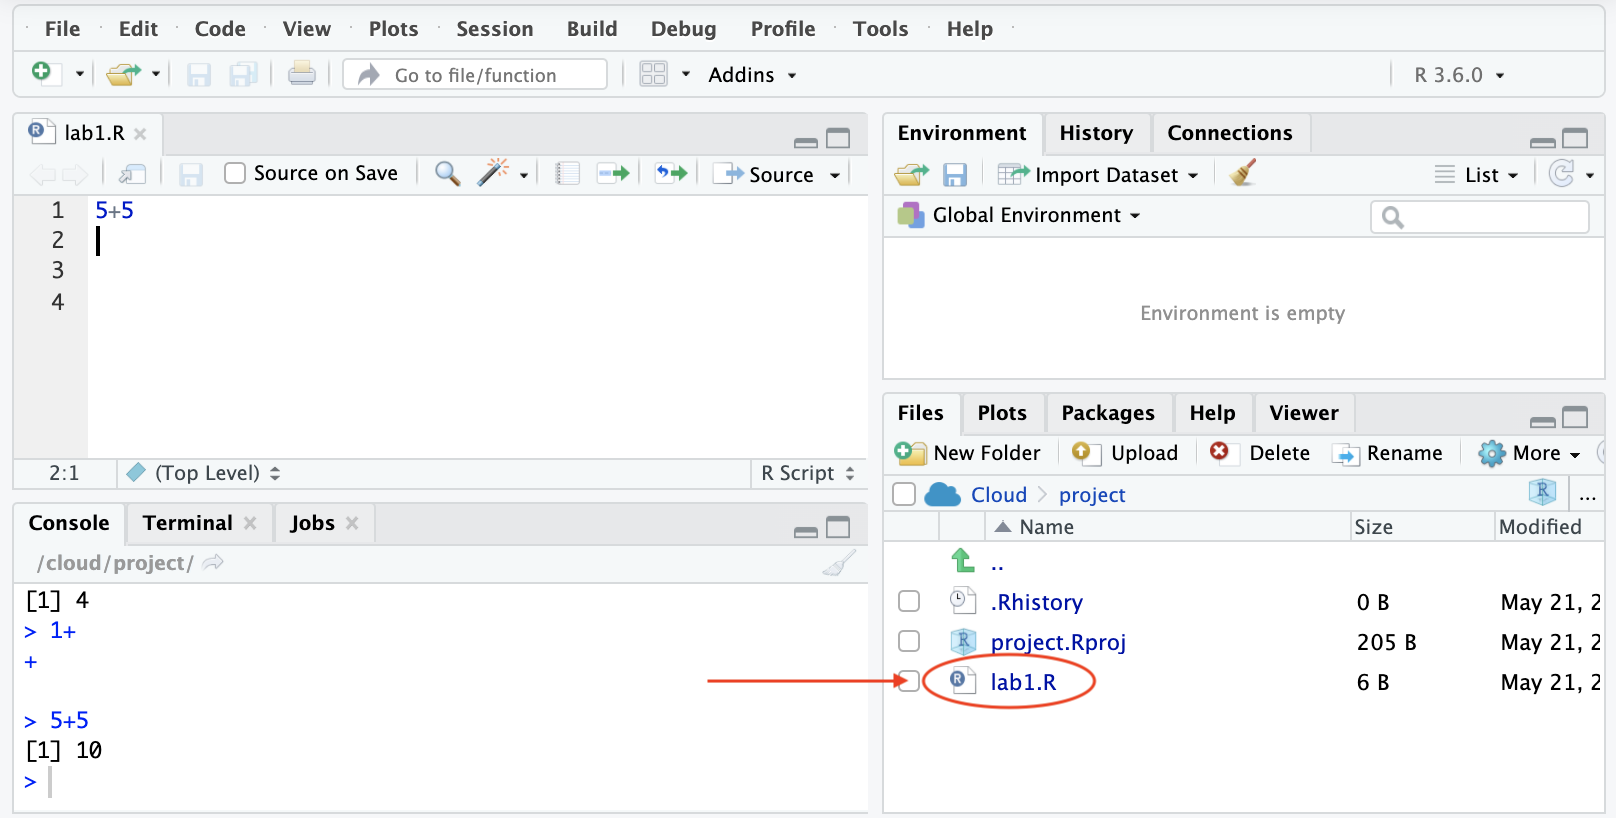
\includegraphics{img/savescript3.png}

\textbf{This script file is a record of your work and is how you will be graded for this lab. Make sure you saved this file and complete the rest of this lab in your `lab1' script.}

Within a script you should include comments to yourself and others using \texttt{\#}. Anything with a \texttt{\#} in front of it will not run. These comments and explanations are an important part of an R script.

For example, type the following in to the script and then run it.

\texttt{\#r\ is\ like\ a\ calculator}

\texttt{2+2}

\texttt{\#Answer\ is\ 4}

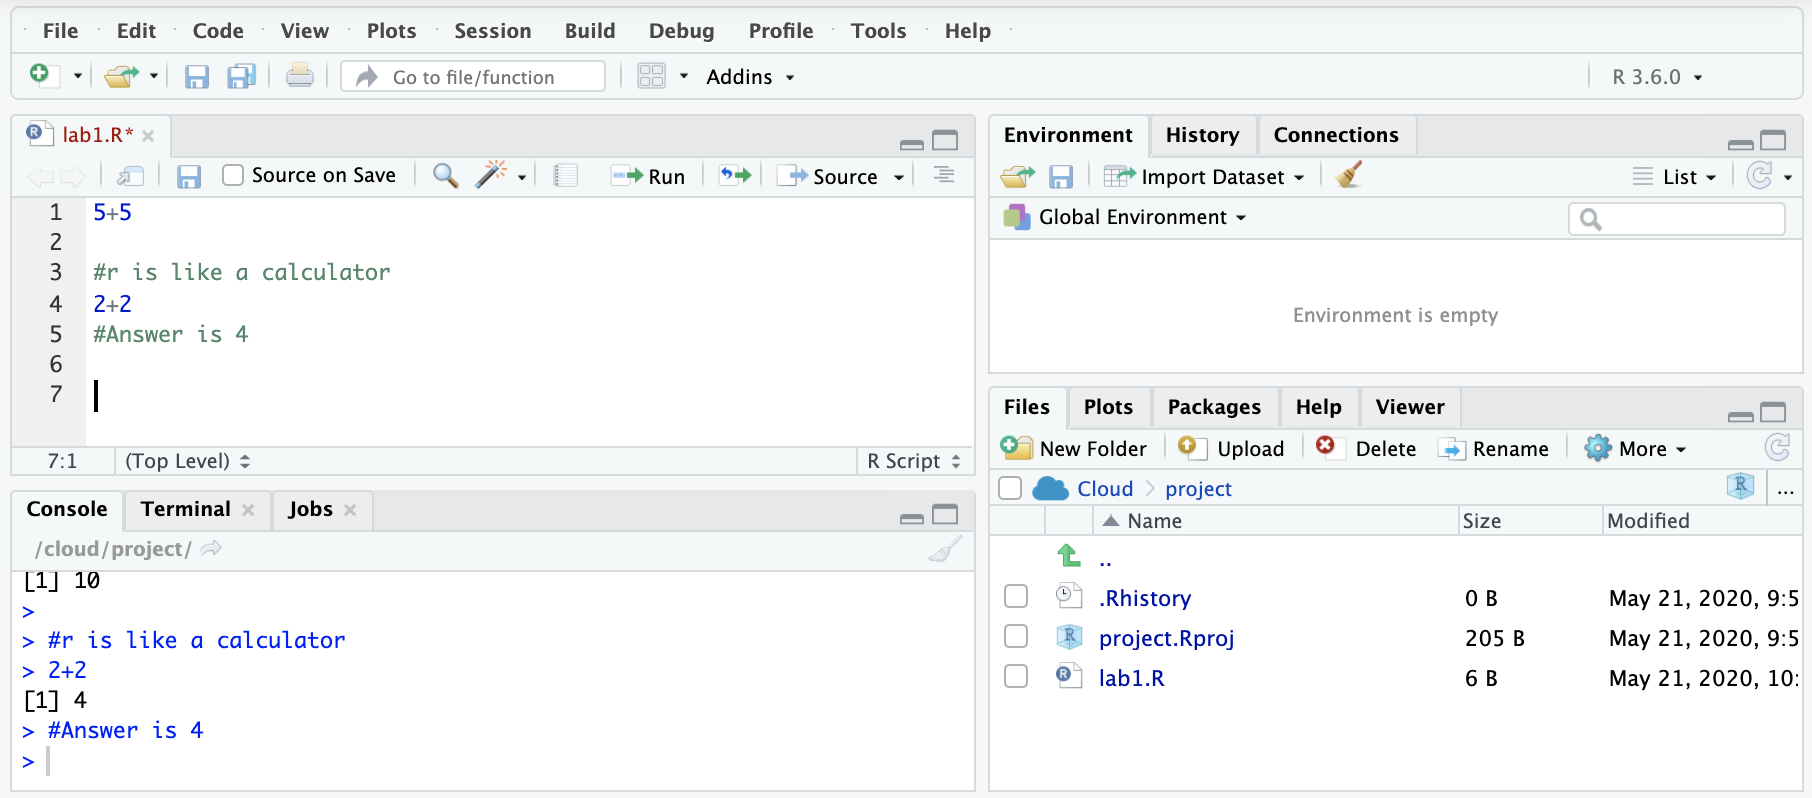
\includegraphics{img/comment.png}

Note that the comments are green in the script.

\hypertarget{environment-and-history}{%
\subsection{Environment and history}\label{environment-and-history}}

In the top right corner of RStudio is the environment and history window. The \textbf{history tab} shows every line of code that has been run in the current session.

The \textbf{environment tab} is where all active \textbf{objects} are listed. An object is something can hold information for later use. The information can be data, values, output, or functions.

Objects are assigned using \texttt{\textless{}-}. Values on the right side of \texttt{\textless{}-} will be assigned to the object on the left side.

For example, let's tell R that the population mean of IQ scores is 100 and the population standard deviation is 15.

To do this use the following code:

\texttt{mu\ \textless{}-\ 100}

\texttt{sigma\ \textless{}-\ 15}

After you run these commands, the objects will now be listed in the environment panel in the top left.

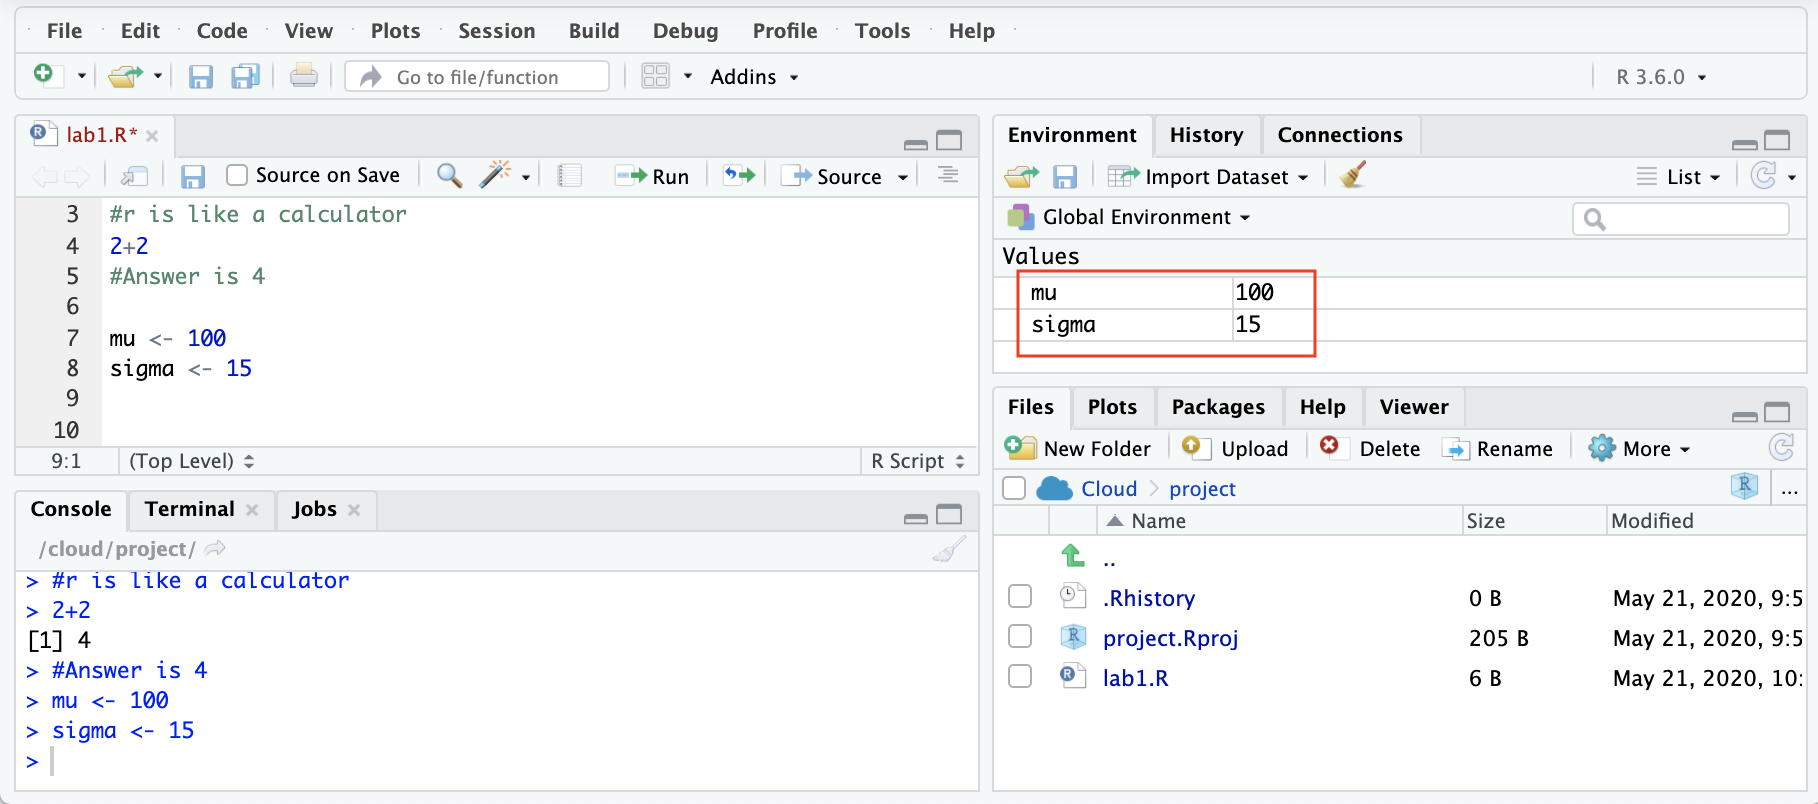
\includegraphics{img/object.png}

The shortcut for making \texttt{\textless{}-} is the ALT and -- key together. (or OPTION and -- on a mac)

\hypertarget{vectors}{%
\subsubsection{Vectors}\label{vectors}}

It is possible to store more than one number in an object. One way to do this is to use a a \textbf{vector}. Assign a set of numbers a vector with the \textbf{combine} function: \texttt{c()}. Do use this, type all the numbers you want to store within the parentheses in a comma separated list.

For example, let's enter IQ scores of students in a small class.

To do this use the following code:

\texttt{classIQ\ \textless{}-\ c(112,\ 115,\ 89,\ 95,\ 101)}

After you run this code,the classIQ vector should appear in the environment.

Here is a picture of what your screen should look like:

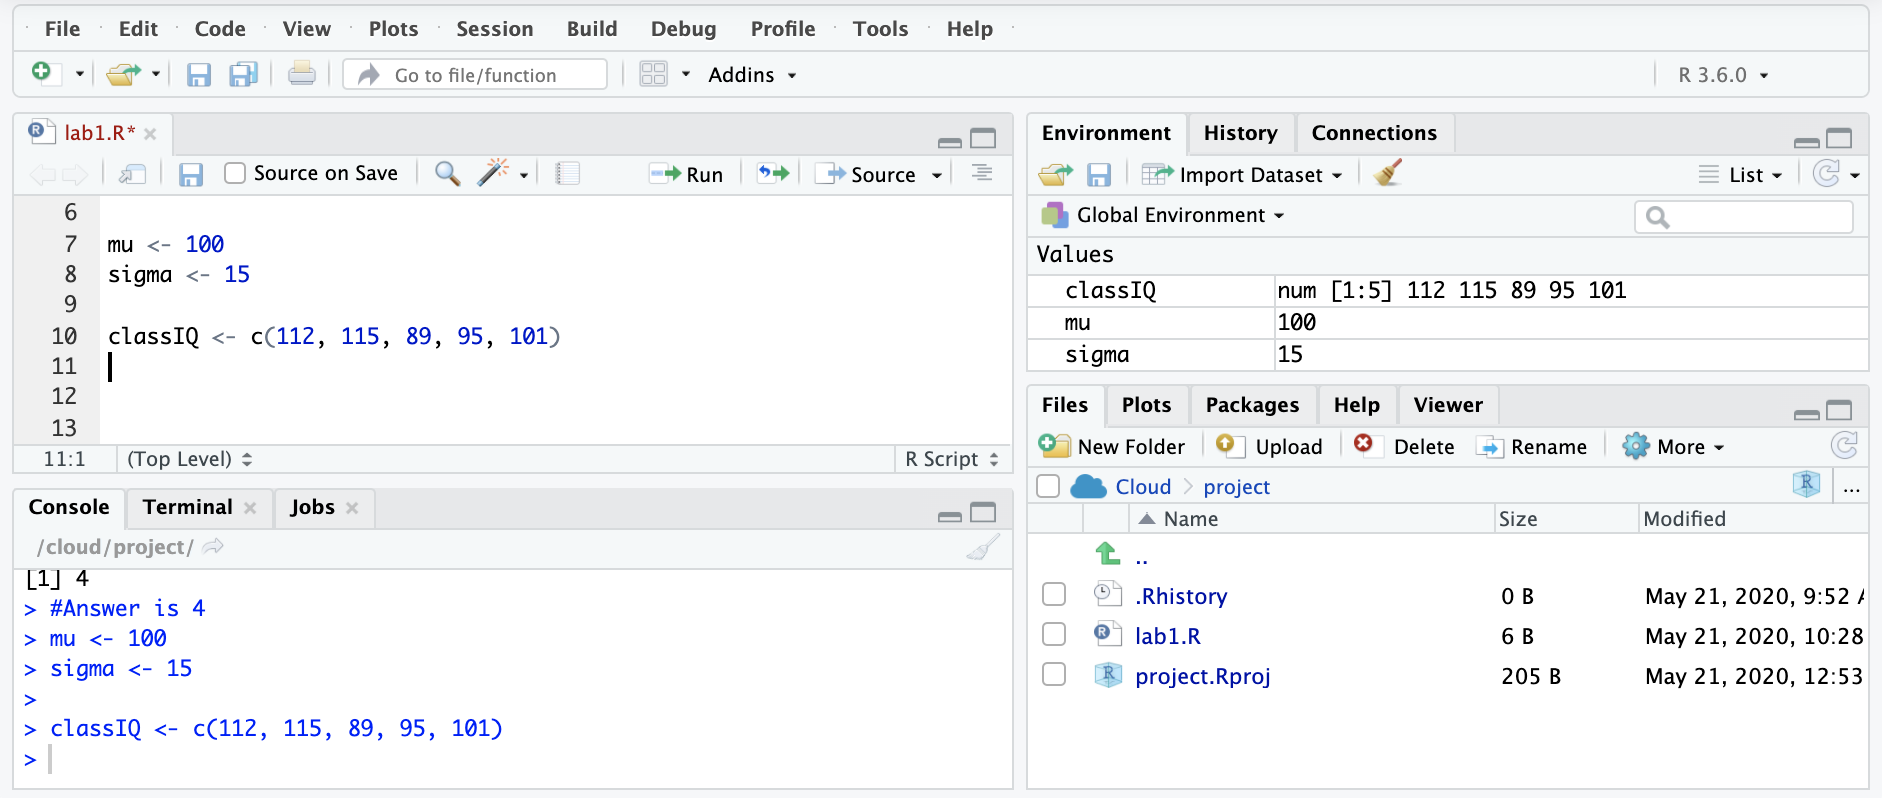
\includegraphics{img/vector.png}

Calculations with vectors apply to all data points.

For example, let's calculate the z-scores for each of the IQ scores.

To do this use the following code:

\texttt{\#get\ z-scores}

\texttt{(classIQ-mu)/sigma}

The results will appear in the console (See the red box in the picture below)

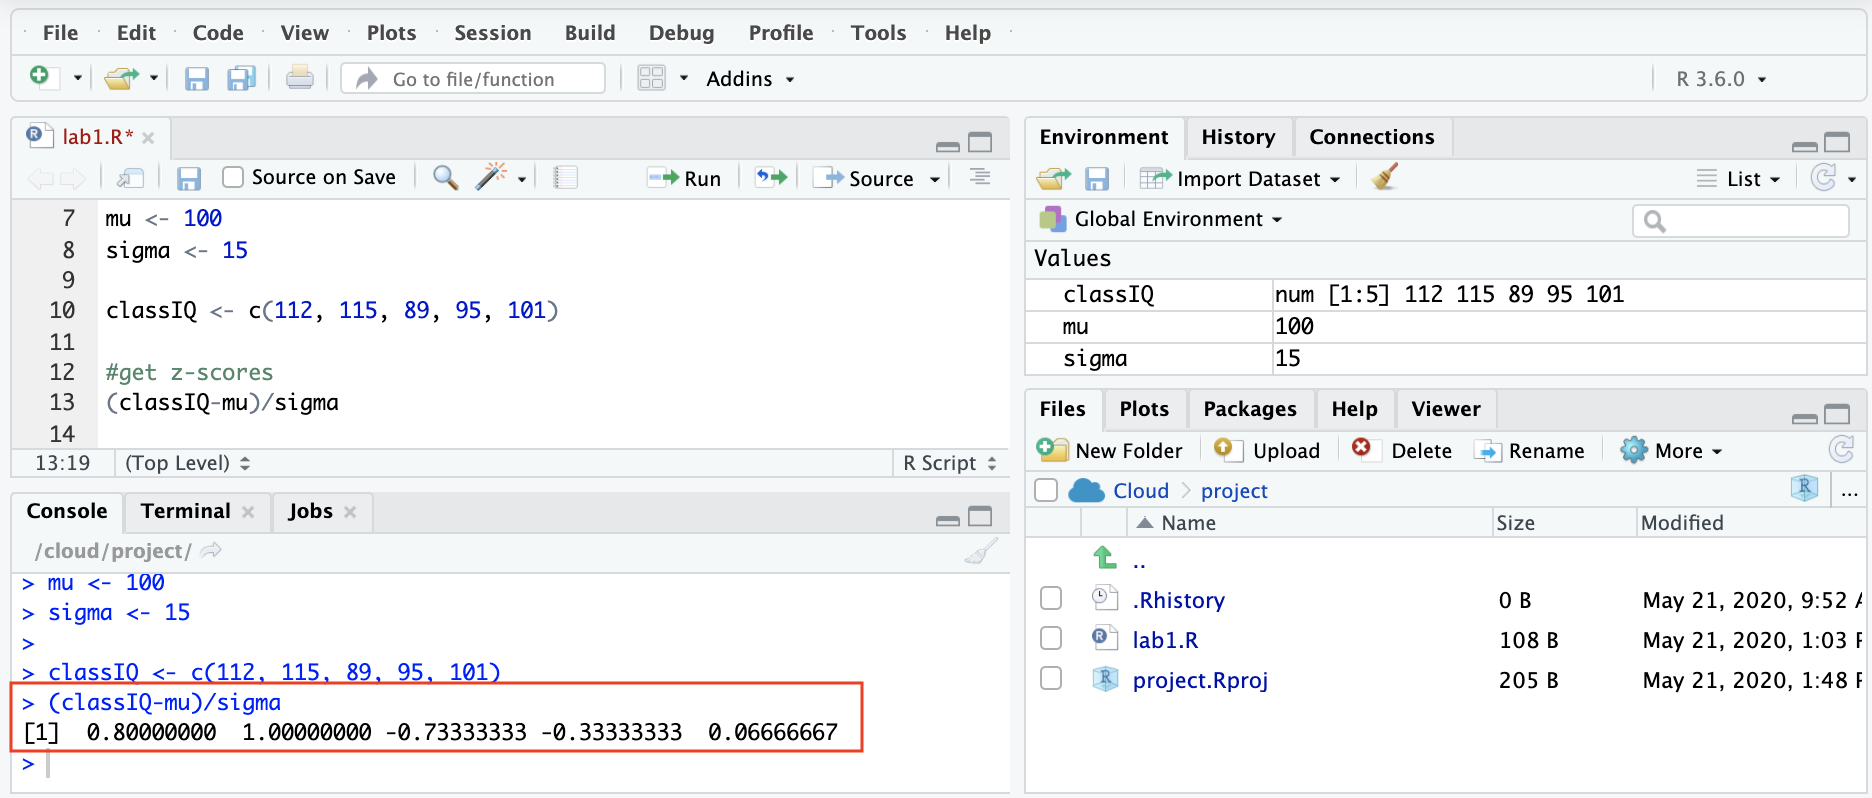
\includegraphics{img/zscores.png}

It is possible to save these answers as a vector using the \texttt{\textless{}-} function.

For example, let's save those zscores in a vector called zscores.

To do this use the following code:

\texttt{zscores\ \textless{}-\ (classIQ-mu)/sigma}

There should now be a vector in the environmnet called zscores.

Here is a picture so that you can check your progress:

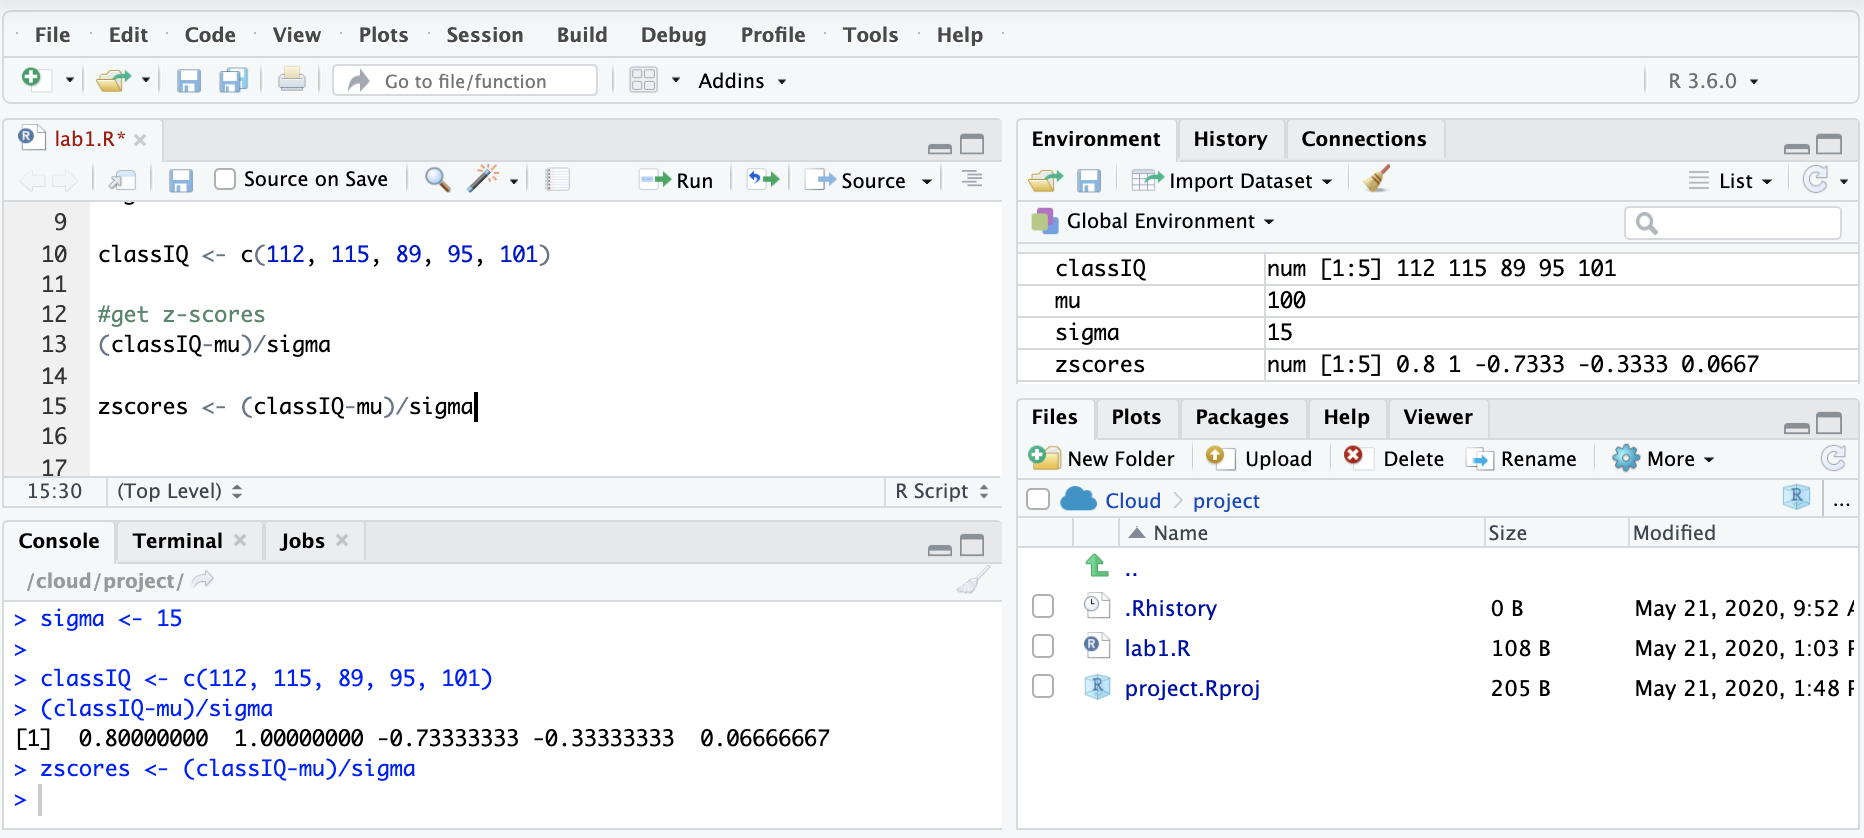
\includegraphics{img/zsaved.png}

\hypertarget{data-frames}{%
\subsubsection{Data frames}\label{data-frames}}

Right now the IQ scores and the z-scores are in separate objects. Variables often need to be in a single object in order to do some basic analyses. You can combine the classIQ and the zscores variable using the \textbf{data.frame} command.

To do this use the following code:

\texttt{iq\ \textless{}-\ data.frame(classIQ,\ zscores)}

\begin{itemize}
\tightlist
\item
  This command takes the form of DatasetName \textless- data.frame(Variable1, Variable2, etc)\\
\item
  The dataset name can be anything you want that you have not already used

  \begin{itemize}
  \tightlist
  \item
    the name must be one word (there cannot be spaces in the name)
  \end{itemize}
\end{itemize}

This object will be listed under data instead of values in the environment panel.

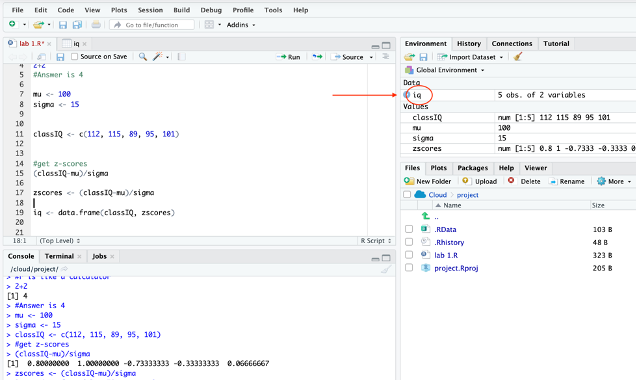
\includegraphics{img/dataframe.png}

Double-click on the word `iq' in the environment panel to look at the dataset that you just created (it is circled in red in the picture above).

A new tab will open with a spreadsheet view of the dataset. When you are done viewing the data, you can close it by click on the `x' next to the name iq.

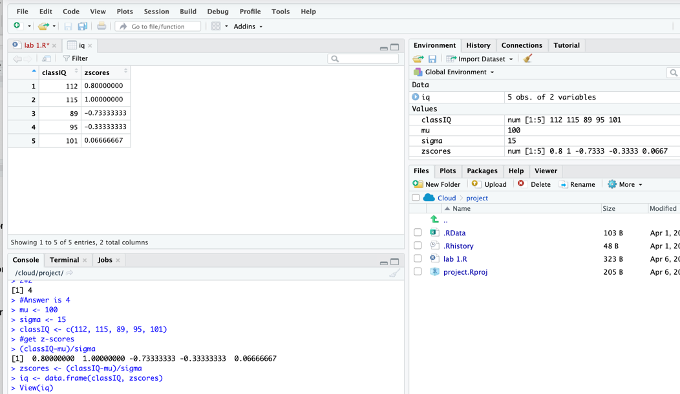
\includegraphics{img/dataframe2.png}

Note that after looking at the dataset this way, the command \texttt{view(iq)} appeared in the console. You can look at the dataset with the \textbf{view} command as well

Finally, when typing the code to create the data frame, you may have noticed that RStudio uses \textbf{predictive text}. This means that RStudio will suggest functions and objects as you type. You should take advantage of this nice feature!

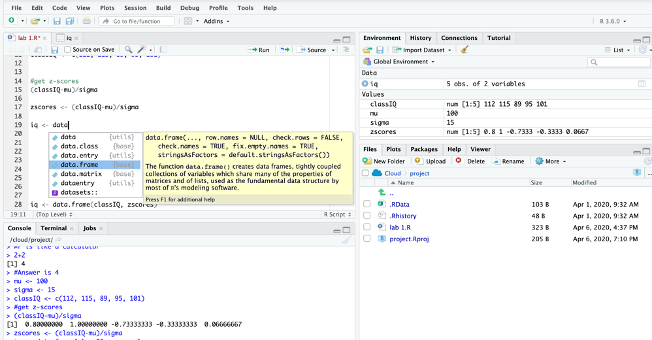
\includegraphics{img/autofill.png}

\hypertarget{importing-data-into-rstudio-cloud}{%
\section{Importing data into Rstudio cloud}\label{importing-data-into-rstudio-cloud}}

In the Introduction section you learned how to assign data to a \textbf{vector} using the \textbf{combine} function.

Another way to assign data to an object is by first entering the data into a spreadsheet (like google sheets or excel) and then import the data into RStudio. This will be our preferred method.

First download the exam2.csv file from d2l.

\hypertarget{upload-the-data-into-rstudio-cloud}{%
\subsection{Upload the data into Rstudio Cloud}\label{upload-the-data-into-rstudio-cloud}}

Then select the UPLOAD button in the files window.

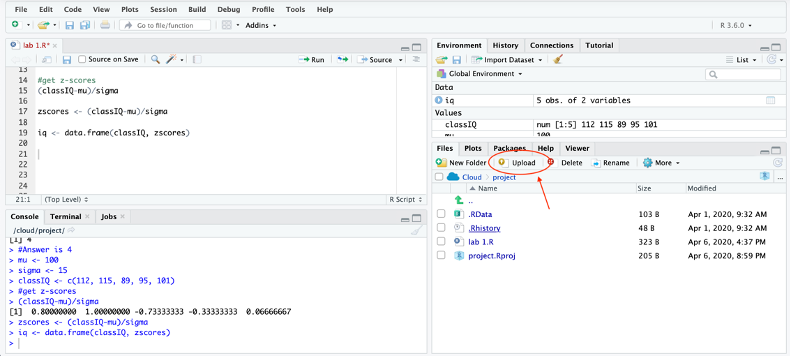
\includegraphics{img/upload.png}

In the Upload Files window, click the CHOOSE FILE button and then navigate to the exam2.csv file on your computer. Then click the OK button.

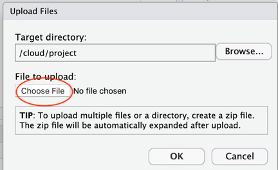
\includegraphics{img/choosefile.png}

The data file should now be listed in the files section of RStudio.

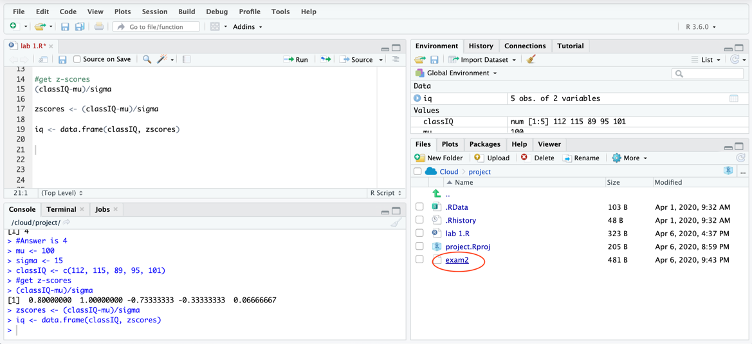
\includegraphics{img/filelist.png}

\hypertarget{import-data}{%
\subsection{Import data}\label{import-data}}

Then you need to import the data into the environment (i.e.~assign the data to an object). This can be done through using point and click options or with code.

\hypertarget{point-and-click}{%
\subsubsection{Point and click}\label{point-and-click}}

First click on the \textbf{IMPORT DATASET} button in the environment panel.

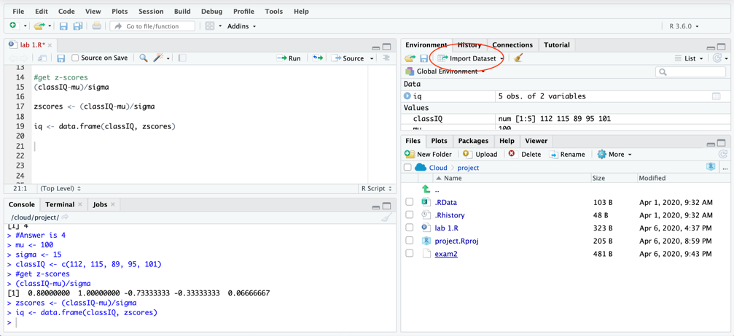
\includegraphics{img/import.png}

Then select the \textbf{`FROM TEXT (READR)'}

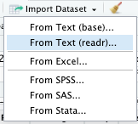
\includegraphics{img/readrbox.png}

The first time you select this -- the following window will appear asking if you would like to install the readr package. Select YES. I will introduce packages in the next section.

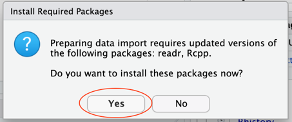
\includegraphics{img/installreadrbox.png}

After you select yes, R will begin downloading the package. This can take a few minutes and will look something like this:

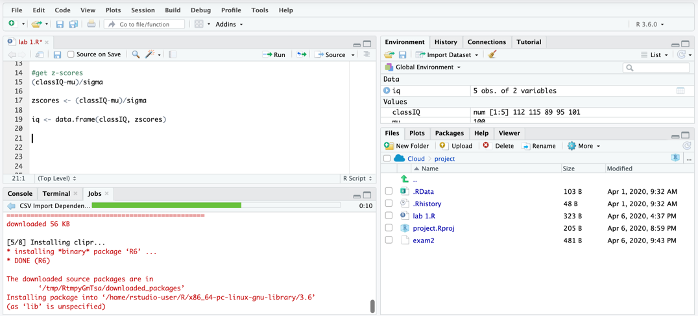
\includegraphics{img/installreadr.png}

It is important to be \emph{patient} here and let the package download completely before you move on to the next step.

When the download is complete, your screen should look like this:

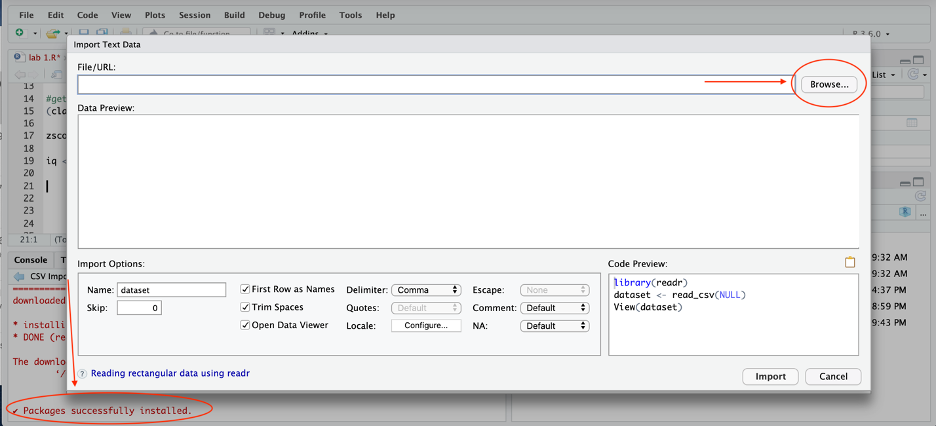
\includegraphics{img/importwindow.png}

Note that you can see that the package was successfully installed in the console in the bottom left. The next time you use readr to import data -- you will not have to download the package first.

Next select the BROWSE button in the top left corner of the import data window.

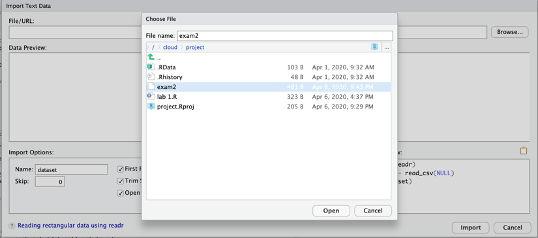
\includegraphics{img/importbrowse.png}

In the choose file window, select `exam2'. And then select OPEN.

The next window should look like this:

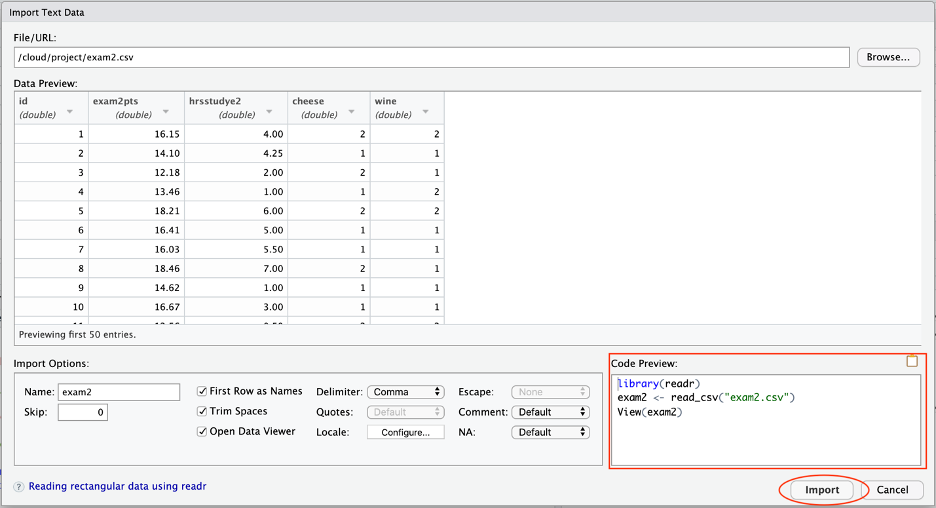
\includegraphics{img/importwindow2.png}

From here you should click the IMPORT button.

But first note the \textbf{Code Preview} box. This is the code you could use to import data (instead of clicking through all these windows). Copy this code before I click the import button and then paste it into your script for your records and in case you need to assign the file to an object again (because it is faster with code).

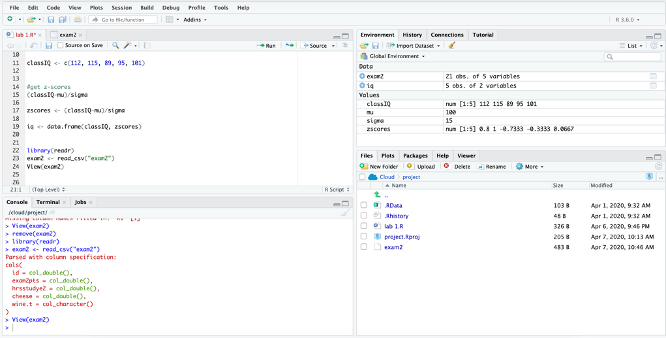
\includegraphics{img/importcomplete.png}

\hypertarget{code}{%
\subsubsection{Code}\label{code}}

Alternatively you could have typed the code that you copy and pasted (and not gone through all of the point and click windows).

\texttt{Library(readr)}\\
\texttt{exam2\ \textless{}-\ read\_cvs("exam2.csv")}

\begin{itemize}
\tightlist
\item
  This command takes the form of DatasetName \textless- read\_cvs(``FILENAME.csv'')\\
\item
  The dataset name can be anything that you have not already used

  \begin{itemize}
  \tightlist
  \item
    the name must be one word (there cannot be spaces in the name)\\
  \end{itemize}
\item
  If you have not installed the readr package, you will have to so first (see the packages chapter for more information)
\end{itemize}

\hypertarget{view-data}{%
\subsubsection{View data}\label{view-data}}

Double click on the word exam2 in the environment panel to look at the dataset.

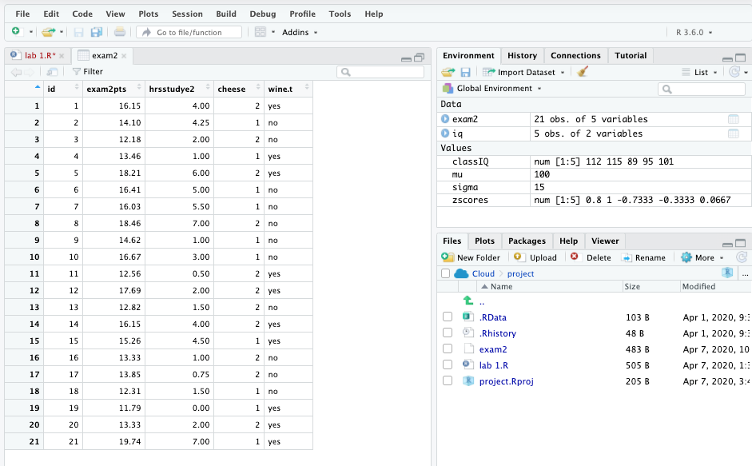
\includegraphics{img/view.png}

Each column is a different variable. Each row is a different participant (in this example a student).\\
- The first column is an arbitrary student ID number -- so that the students' identity is protected.\\
- The second column is exam points earned by the students out of 20 (this is real data from a Fall 2019 class).\\
- The third column is the number of hours the students studied for the exam (this is made up data).\\
- The fourth column is whether or not students ate cheese the night before the exam (1 = no; 2 = yes\ldots{} also made up data).\\
- The last column is data on whether or not students drank wine the night before the exam (1 = no; 2 = yes\ldots{} also made up data).

\hypertarget{packages}{%
\chapter{Packages}\label{packages}}

\textbf{NOTE:} Please open a new script and call it lab 2 (or week 2) for the replication of this chapter and the picturing data chapter assignment.

\textbf{Base R} refers to the functions that automatically come with R. But many people build on top of Base R to make R better. The way they do this is through \textbf{packages}, which contain new R functions. There are thousands of packages available that can do fancy things like quickly compute descriptive statistics and create APA style tables (and much much more).

The first time you use a package, you need to install it. Once a package is installed, you will need to tell R that you want to use it by loading it. You will need to load any packages you want to use each time you open the R program. (I am not exactly sure how this works in the RStudio cloud because it does not seem to shut down when you close out of the RStudio cloud website. See the Restarting R section below for a work around.)

That is, you only have to install a package once. You will have to load a package every time you want to use it.

\hypertarget{installing-packages}{%
\section{Installing packages}\label{installing-packages}}

The first time you use a package, you need to install it. We actually did this once already while importing data! This time let's learn more about the process.

In RStudio, packages can be installed through point and click (GUI) or with code.

\hypertarget{installing-packages-using-point-and-click-gui}{%
\subsection{Installing packages using point and click (GUI)}\label{installing-packages-using-point-and-click-gui}}

Let's first install a package called \textbf{Tidyverse}. Tidyverse was created by Hadley Wickham and his team with the aim of making various aspects of data analysis in R easier. It is actually collection of packages that include a lot of functions (e.g., subsetting, transforming, visualizing) that many people think of as essential for data analysis. (See the tidyverse website for additional information: \url{https://www.tidyverse.org}).

To install a package with GUI go to the top bar menu:

TOOLS -\textgreater{} INSTALL PACKAGES

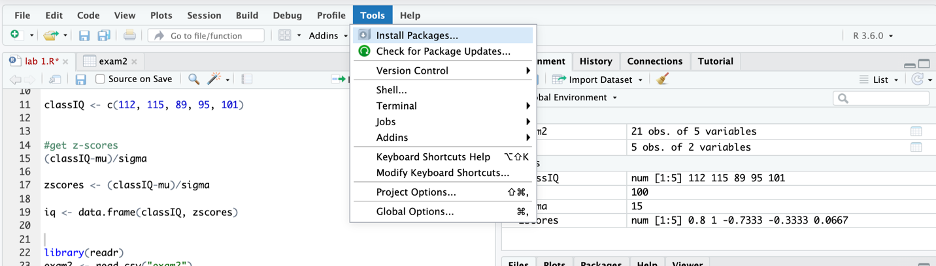
\includegraphics{img/instpacktools.png}

In the install packages window, type the name of the package you would like to install. For example, type \texttt{tidyverse} in the packages box.

Then click INSTALL.

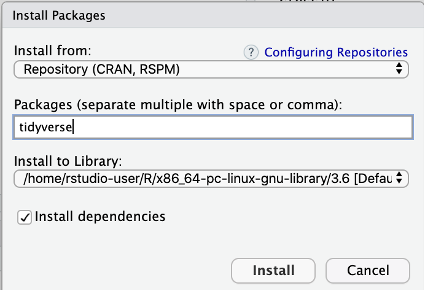
\includegraphics{img/instpackguitidy.png}

Again, installing a package can be a little slow on the RStudio cloud. Please be patient (maybe this is a good time to stretch your legs, refill your beverage, let the dog out, etc.)

Your screen should look like this when it is starting to install:

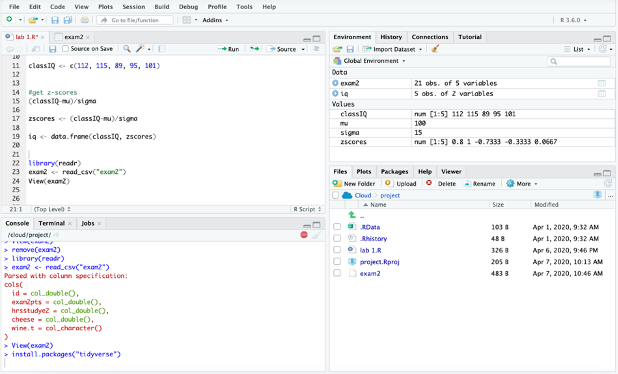
\includegraphics{img/instload1.png}

It should look like this when it is in the process of installing:

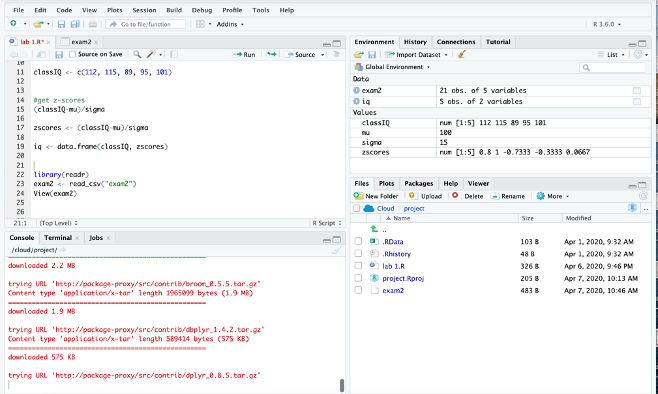
\includegraphics{img/instload2.png}

And then this when the installation is complete:

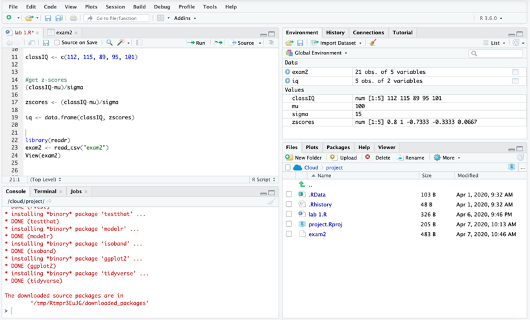
\includegraphics{img/instload3.png}

Do not proceed until the console says the package has been installed.

\hypertarget{installing-packages-using-code}{%
\subsection{Installing packages using code}\label{installing-packages-using-code}}

You can also install a package using this code:\\
\texttt{install.packages()}

To install tidyverse, for example, you would use this code:\\
\texttt{install.packages("tidyverse")}~\\
- Note that the word tidyverse is in quotes

But do not run this code -- as you have already installed it with GUI.

Instead, let's install a package called psych using the \texttt{install.packages} command. The \textbf{psych package} is a package for personality, psychometric, and psychological research. It has been developed at Northwestern University (maintained by William Revelle) to include useful functions for personality and psychological research.

To install this package, use following command:\\
\texttt{install.packages("psych")}

Your screen should look like this when the package is completely installed:\\
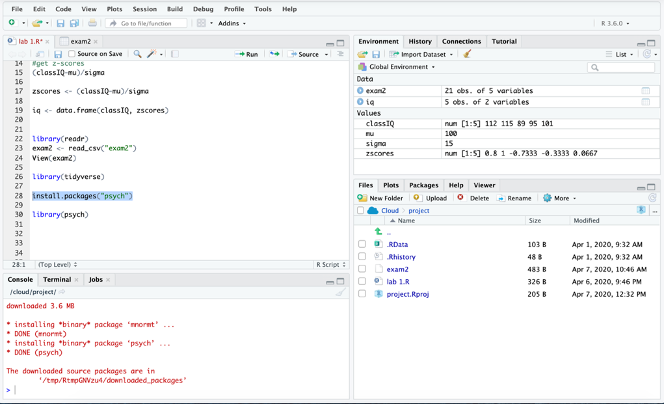
\includegraphics{img/instpsyc.png}

Remember that installing packages is the first step to using them and they only have to be installed once.

Next let's learn how to load packages, so that you can use thier functions.

\hypertarget{loading-packages}{%
\section{Loading Packages}\label{loading-packages}}

Installing a package is only the first step.

\textbf{In order to use a package, it must be loaded first.}

Packages can only be loaded with code. Packages need to be loaded every time you open the RStudio program. Most people's R scripts begin with the code that load packages.

When you have the Rstudio program installed on your computer this is straight forward (either the program is open or closed). This is less clear with Rstudio cloud because it does not seem to always shut down when you close the web browser site. (Please see the section on restarting Rstudio in the misc section below for a work around.)

The command to load a package is:\\
\texttt{library()}

For example, load the tidyverse package with this:\\
\texttt{library(tidyverse)}

After you run this code, your screen should look like this:

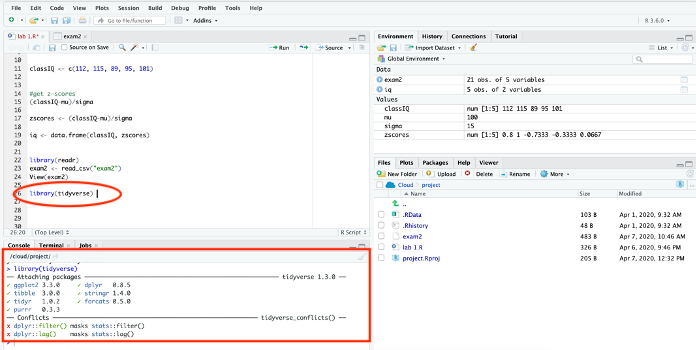
\includegraphics{img/loadtidy.png}

The console shows that the Tidyverse package has been loaded (don't worry about the conflicts for now).

Next let's load the psych package using this command:\\
\texttt{library(psych)}

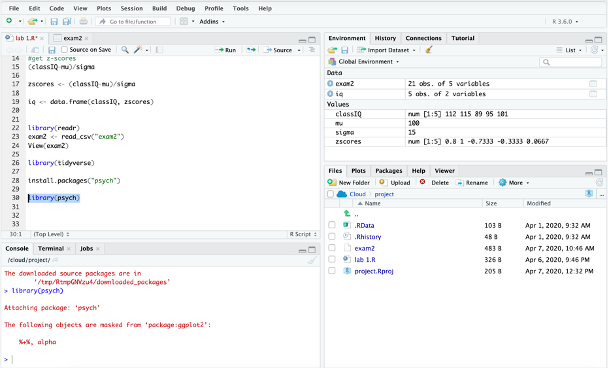
\includegraphics{img/loadpsyc.png}
Again, don't worry about the warning about masked functions for now.

\hypertarget{misc}{%
\section{Misc}\label{misc}}

You can get additional information using the \texttt{help()} function and \texttt{?} help operator in R. They both provide access to documentation pages for all functions and packages.

For example, use the following code to get more information about Tidyverse:\\
\texttt{?tidyverse}

Or this command to get more information about Psych:

\texttt{help(psych)}

\hypertarget{restarting-r}{%
\subsection{Restarting R}\label{restarting-r}}

Because it is unclear whether Rstudio completely turns off when you close the website, you could restart the R session to simulate the act of closing and reopening the Rstudio program (like you could if it were installed on your computer).

To do this, in the drop down menu go to:

SESSION -\textgreater{} RESTART R

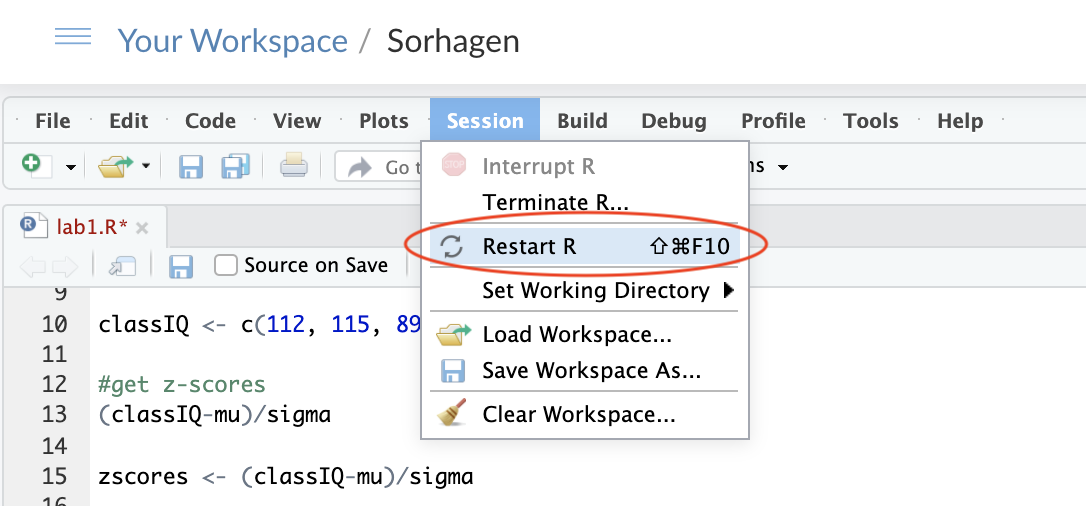
\includegraphics{img/restart.png}

When you restart the R session, everything in the script, environment, console, and files will remain.

All packages that were loaded will be cleared, so you will have to reload them if you want to use them.

If something is not working like it is suppose to (and you have checked for type-os), try restarting the R session. It could be that the functions of one package conflict or mask the functions of another package.

  \bibliography{book.bib,packages.bib}

\end{document}
